\documentclass{article}
\usepackage[parfill]{parskip}
\usepackage[absolute]{textpos}
\usepackage{float}
\usepackage{graphicx}
\usepackage[T1]{fontenc}
\usepackage[scaled]{helvet}
\usepackage{lscape}
\usepackage{courier}
\renewcommand*\familydefault{\sfdefault}
\usepackage[left=1in,top=1in,bottom=1.25in,right=1in]{geometry}
\usepackage{color}
\usepackage{fancyhdr,lastpage}
\pagestyle{fancy}
\usepackage{listings}
\usepackage{verbatim}
\rhead{\scriptsize \proptitle}
%\chead{Middle top}
\setlength{\headheight}{45pt}
\newenvironment{changemargin}[2]{%
\begin{list}{}{%
\setlength{\topsep}{0pt}%
\setlength{\leftmargin}{#1}%
\setlength{\rightmargin}{#2}%
\setlength{\listparindent}{\parindent}%
\setlength{\itemindent}{\parindent}%
\setlength{\parsep}{\parskip}%
}%
\item[]}{\end{list}}
%\newcommand{\CR}{43}
\lhead{
\includegraphics[scale=.55]{logonew.pdf}}%\\\smallskip\scriptsize  CR-\CR}

\fancyfoot[C]{Page \thepage\ of \pageref{LastPage}}
\usepackage[colorlinks=true,linkcolor=black,urlcolor=blue]{hyperref}

\newcommand{\topic}{Data testing summary}
\newcommand{\proptitle}{Pharmacometrics TFL Generator v1.0.0 qualification}
\newcommand{\testinglog}{tables-testing-log-complete.pdf}

\newcommand{\propversion}{metworx-2.1}
\newcommand{\nmqualversion}{8.3.3}
\newcommand{\nmversion}{7.3}
\newcommand{\openbugsversion}{3.2.3}
\newcommand{\rversion}{3.2.2}
\newcommand{\rstudioversion}{0.98.1102}
\newcommand{\mrgqualversion}{0.2.6}

\newcommand{\piranajsversion}{1.20}
\newcommand{\JAGSversion}{3.4.0}
\newcommand{\stanversion}{2.6.0}
\newcommand{\psnversion}{4.2.0}

\newcommand{\metworx}{Metworx\texttrademark}
\newcommand{\tfl}{Pharmacometrics TFL Generator}

\usepackage{lscape}
\usepackage{pdfpages}
\begin{document}

\vspace*{1cm}
\begin{center}
{\large CONFIDENTIAL} 


\vspace*{1cm}


\vspace*{1cm}

{\Large \topic}
\vspace{3.0cm}
\end{center}

\newpage
\vspace*{1cm}
\begin{center}
\vspace{3.0cm}

\begin{tabular}{|l|l|}\hline
Testing performed by &   Dan Polhamus\\
                      &  Senior Scientist \\
                      &  Metrum Research Group LLC \\
                      &  2 Tunxis Road, Suite 112\\
                      &  Tariffville, CT\\
                      &  Phone:  \\
                      &  Fax: 860-372-7988 \\
                      &  Email:  \\\hline
 (Sign and print name) & \\
                       & \\
                       & \\\hline
Dates (YYYY-MM-DD)     &               \\\hline



\end{tabular}

\end{center}

\newpage

\section*{Testing log}

\includepdf[pages=-]{\testinglog}

\newpage


\section*{Appendix}

\subsection*{Screenshots}

\begin{figure}[H]
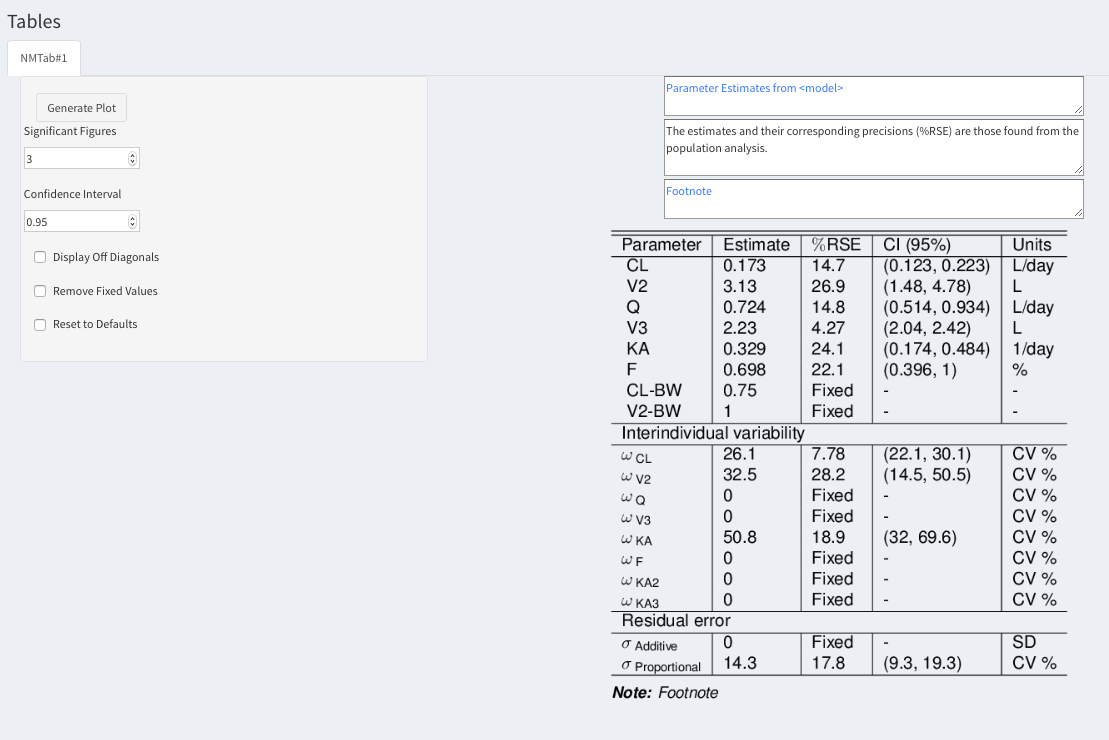
\includegraphics[width=.8\textwidth]{screencaps/24-2-1.png}
\caption{RID: 24 Test ID: 2}
\end{figure}

\begin{figure}[H]
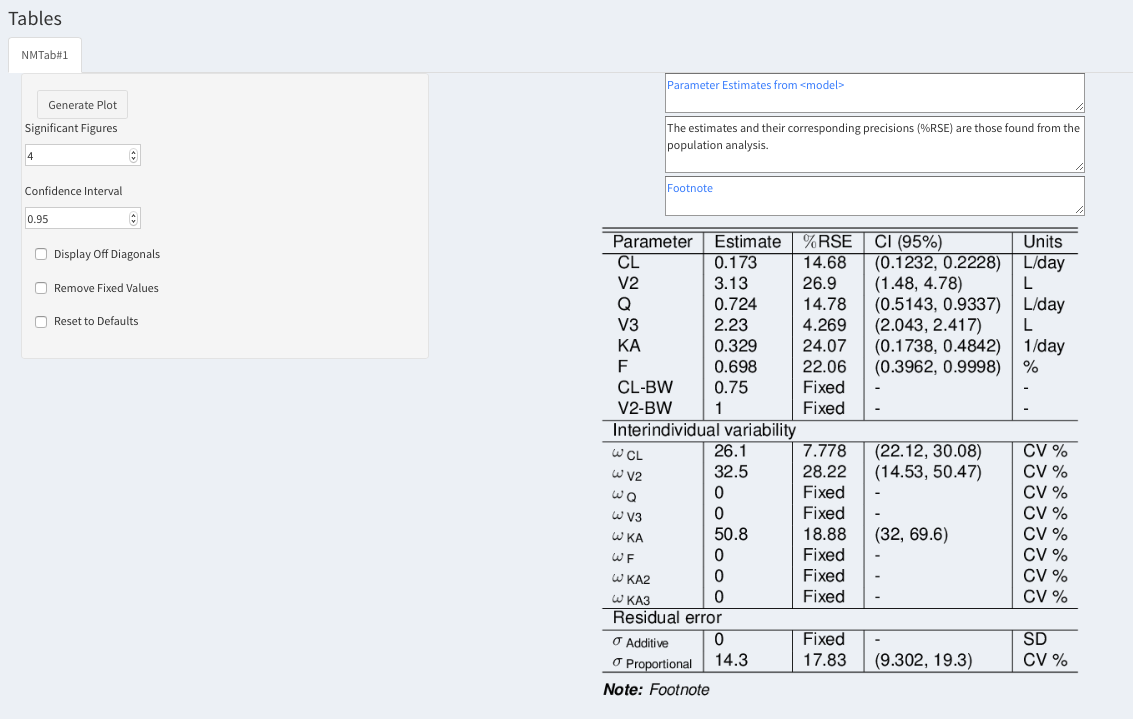
\includegraphics[width=.8\textwidth]{screencaps/24-2-2.png}
\caption{RID: 24 Test ID: 2}
\end{figure}


\begin{figure}[H]
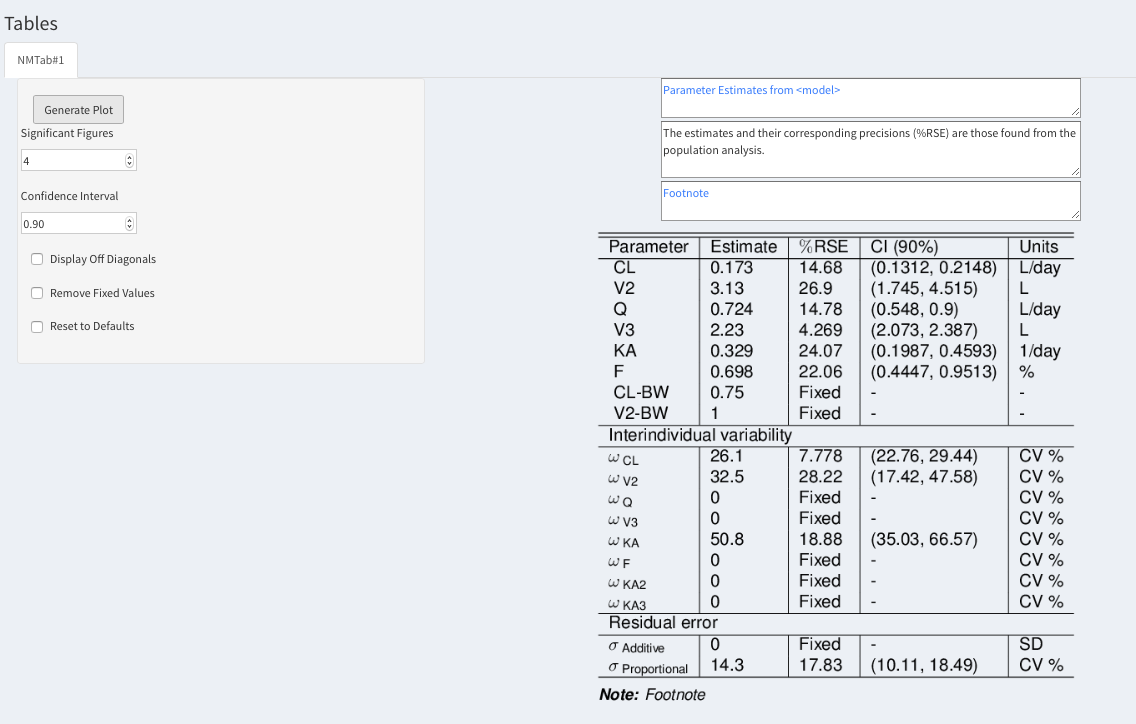
\includegraphics[width=.8\textwidth]{screencaps/24-2-3.png}
\caption{RID: 24 Test ID: 2}
\end{figure}

\begin{figure}[H]
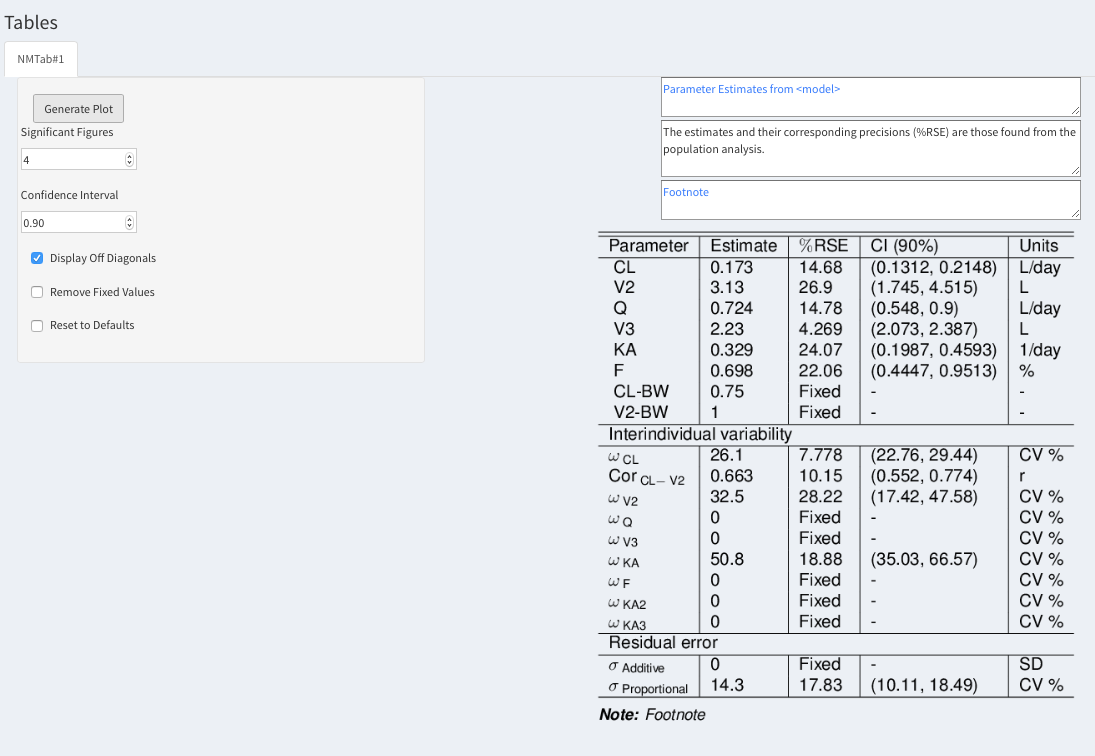
\includegraphics[width=.8\textwidth]{screencaps/24-2-4.png}
\caption{RID: 24 Test ID: 2}
\end{figure}


\begin{figure}[H]
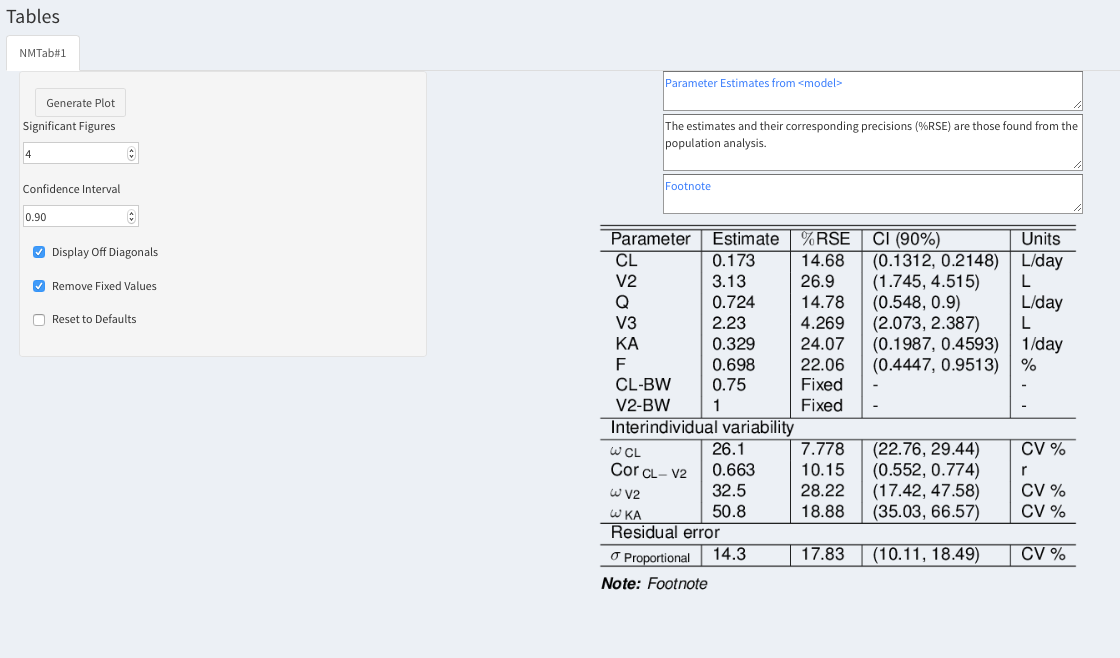
\includegraphics[width=.8\textwidth]{screencaps/24-2-5.png}
\caption{RID: 24 Test ID: 2}
\end{figure}

\begin{figure}[H]
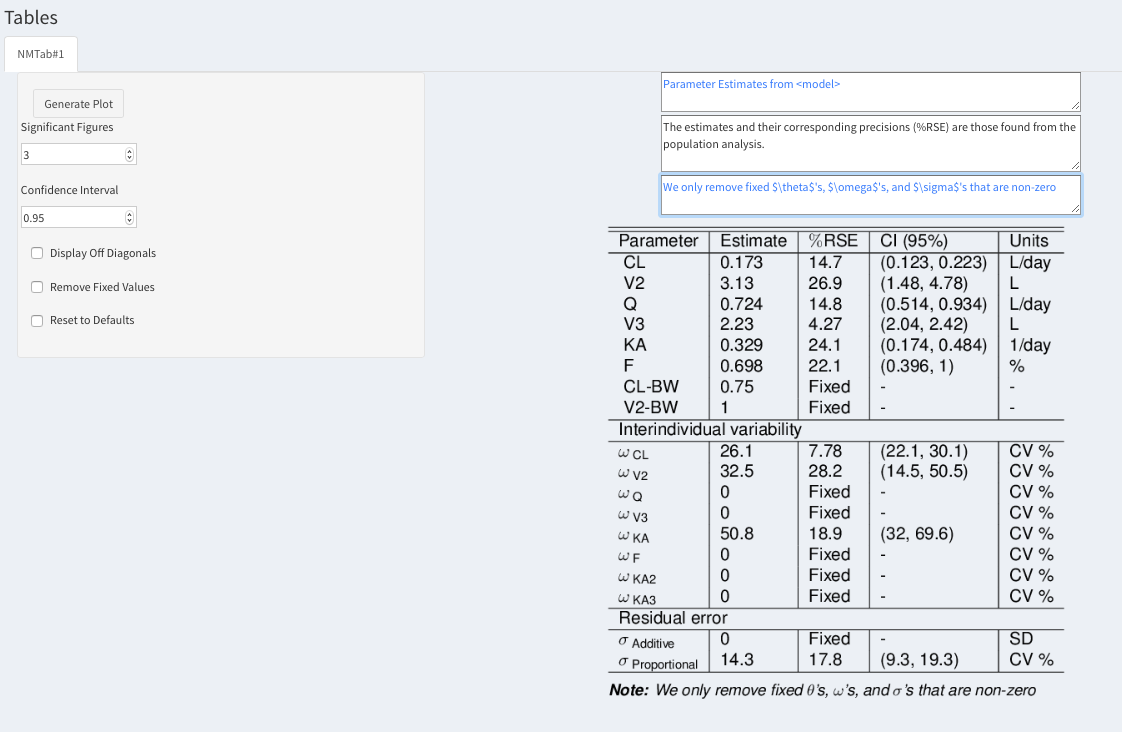
\includegraphics[width=.8\textwidth]{screencaps/24-3-1.png}
\caption{RID: 24 Test ID: 3}
\end{figure}

\begin{figure}[H]
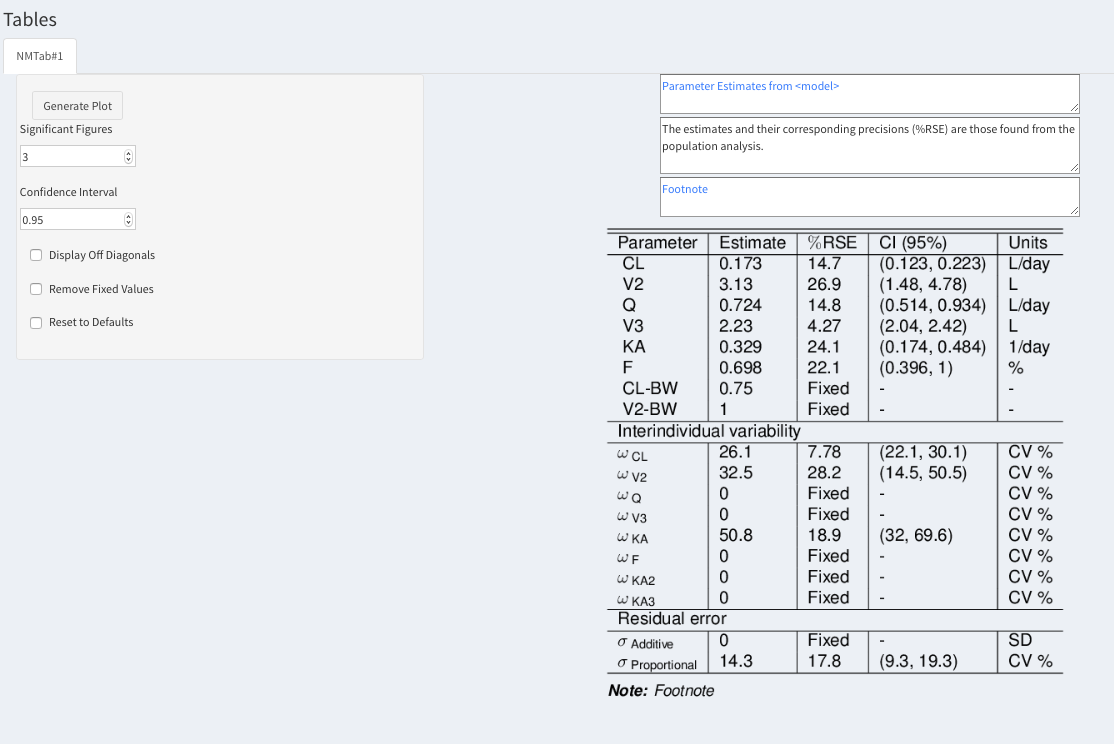
\includegraphics[width=.8\textwidth]{screencaps/24-4-1.png}
\caption{RID: 24 Test ID: 4}
\end{figure}

\begin{figure}[H]
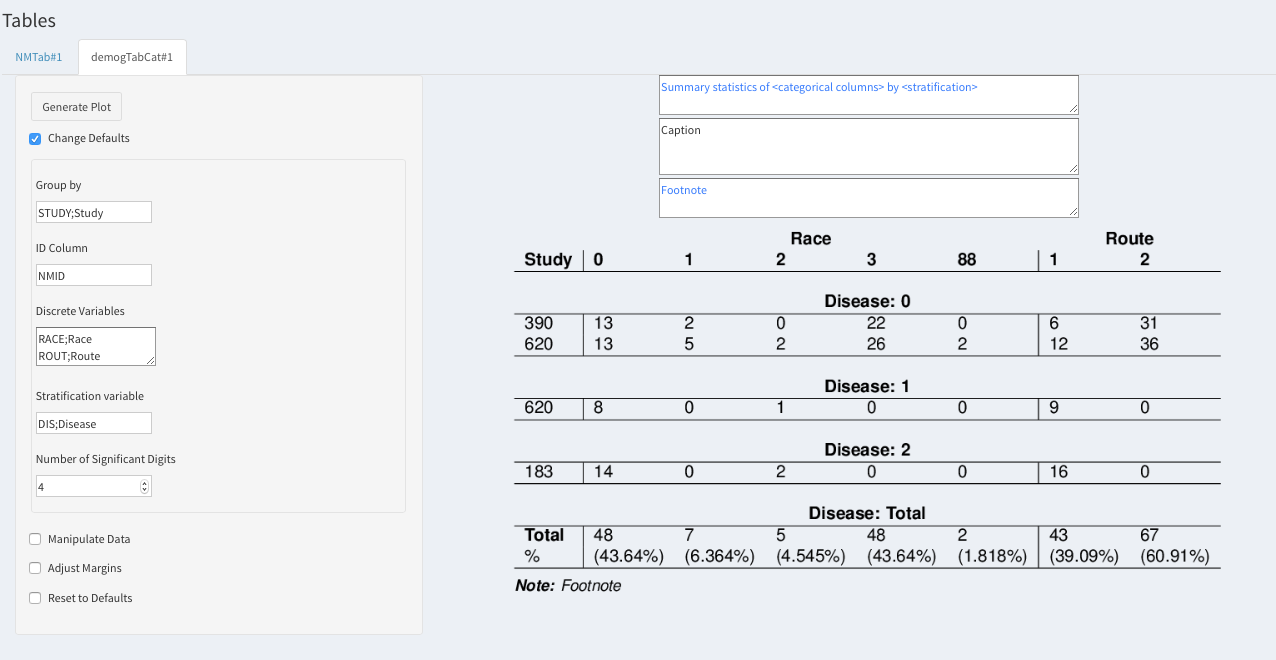
\includegraphics[width=.8\textwidth]{screencaps/25-2-1.png}
\caption{RID: 25 Test ID: 2}
\end{figure}

\begin{figure}[H]
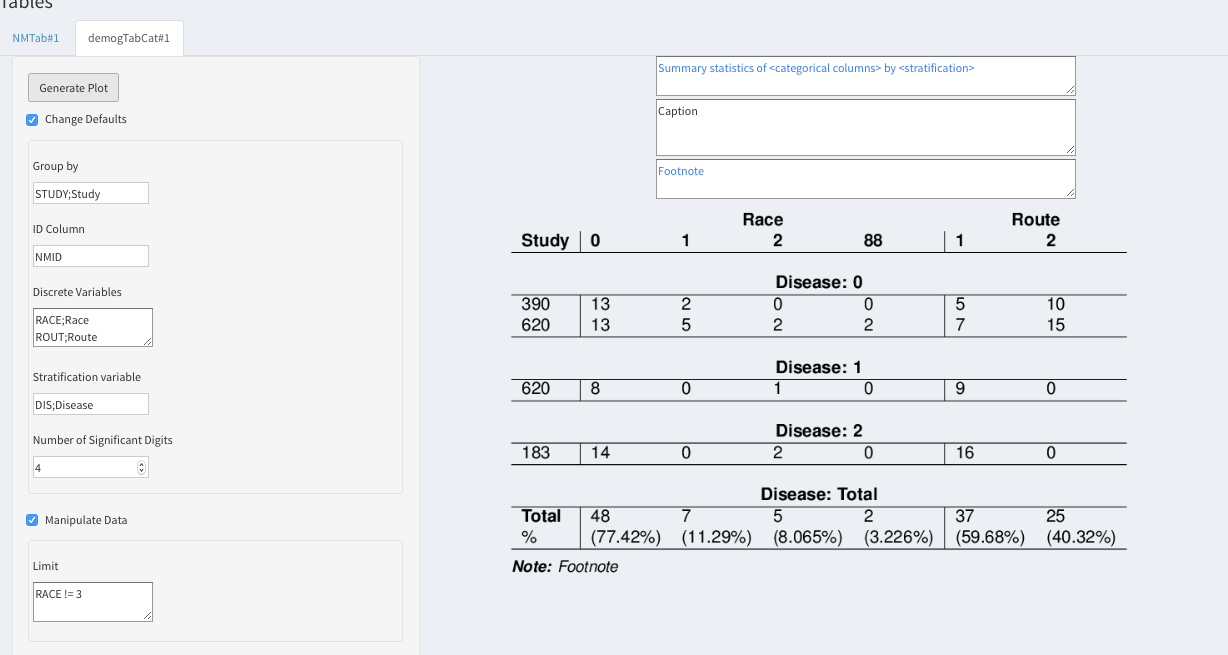
\includegraphics[width=.8\textwidth]{screencaps/25-2-2.png}
\caption{RID: 25 Test ID: 2}
\end{figure}

\begin{figure}[H]
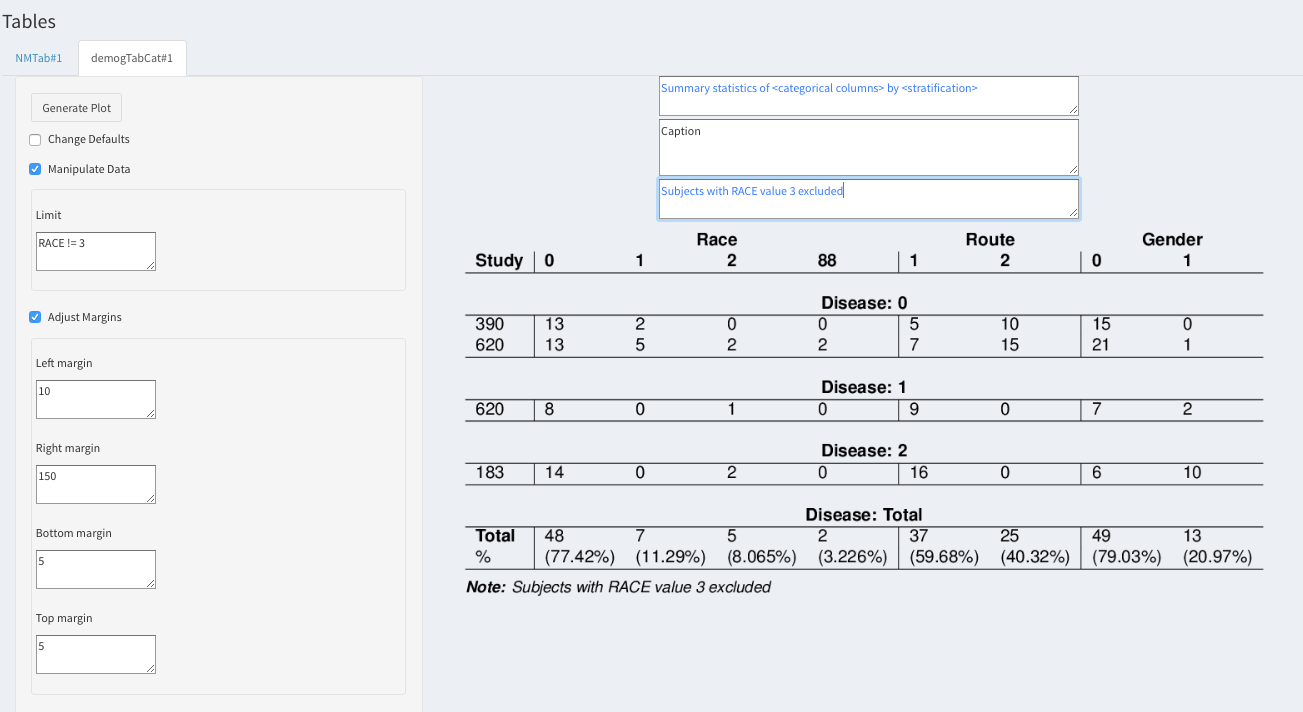
\includegraphics[width=.8\textwidth]{screencaps/25-3-1.png}
\caption{RID: 25 Test ID: 3}
\end{figure}

\begin{figure}[H]
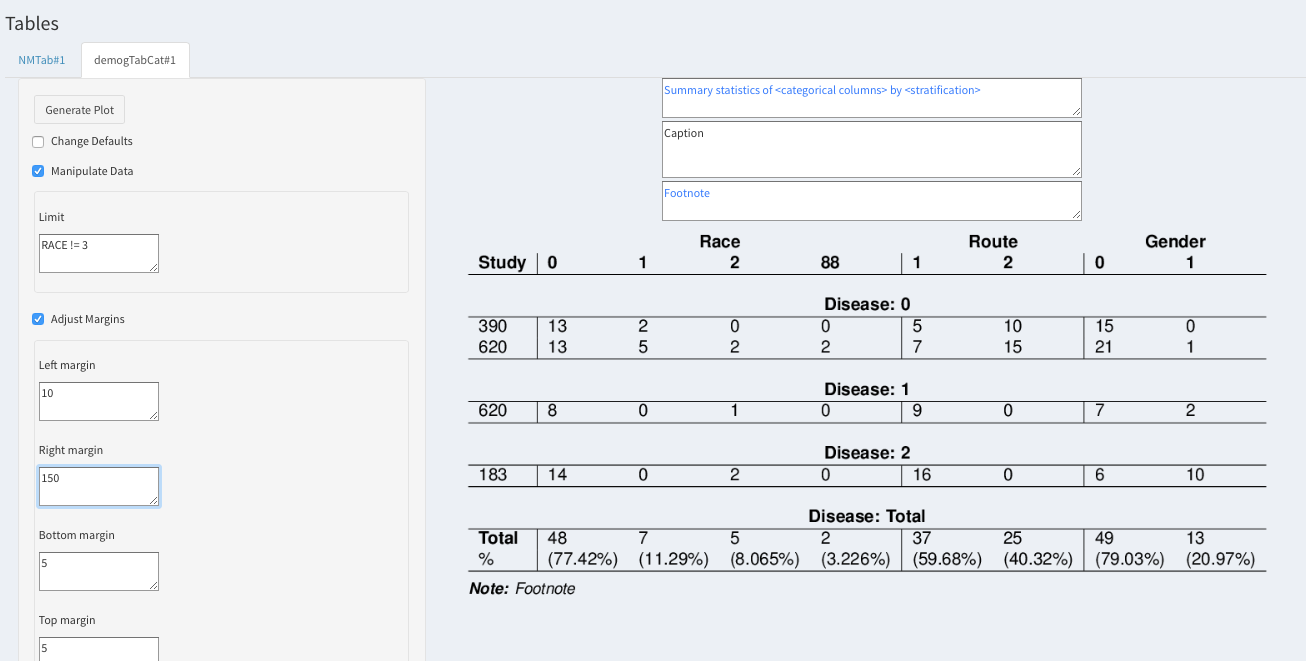
\includegraphics[width=.8\textwidth]{screencaps/25-4-1.png}
\caption{RID: 25 Test ID: 4}
\end{figure}

\begin{figure}[H]
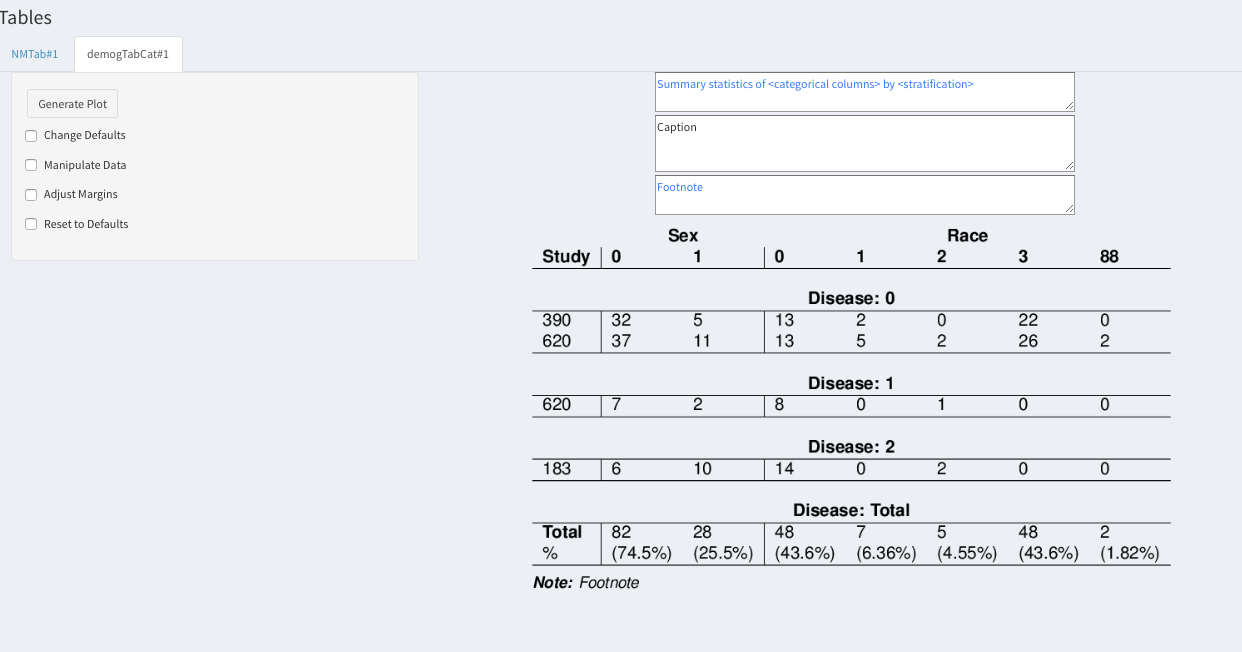
\includegraphics[width=.8\textwidth]{screencaps/25-6-1.png}
\caption{RID: 25 Test ID: 6}
\end{figure}


\begin{figure}[H]
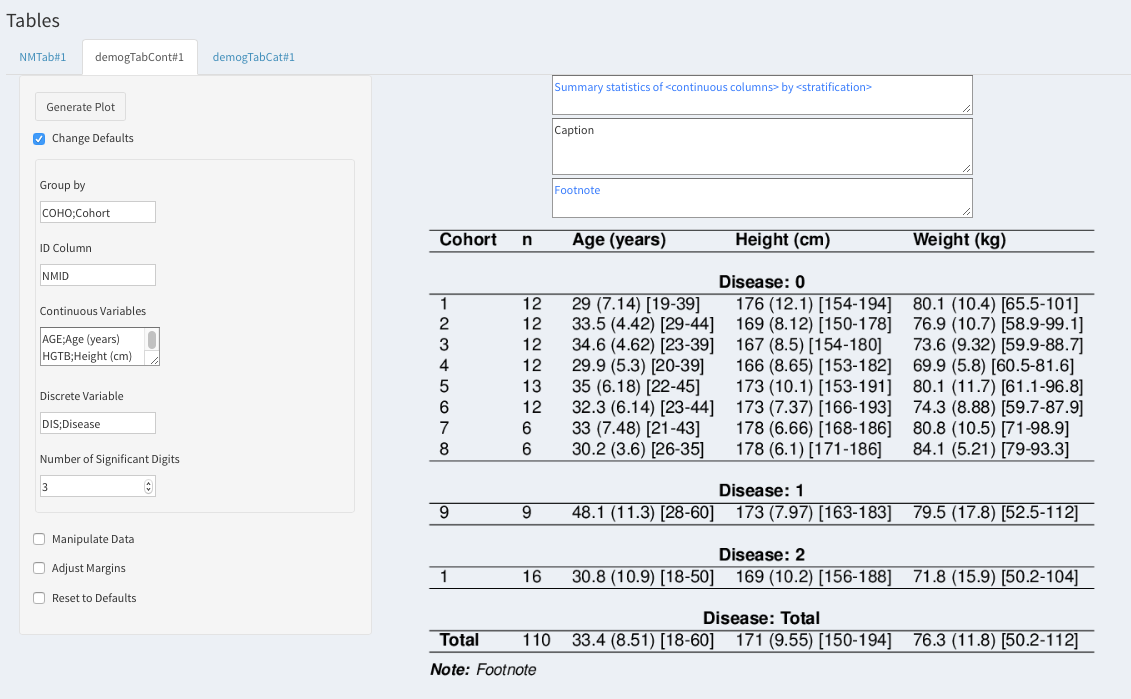
\includegraphics[width=.8\textwidth]{screencaps/26-2-1.png}
\caption{RID: 26 Test ID: 2}
\end{figure}


\begin{figure}[H]
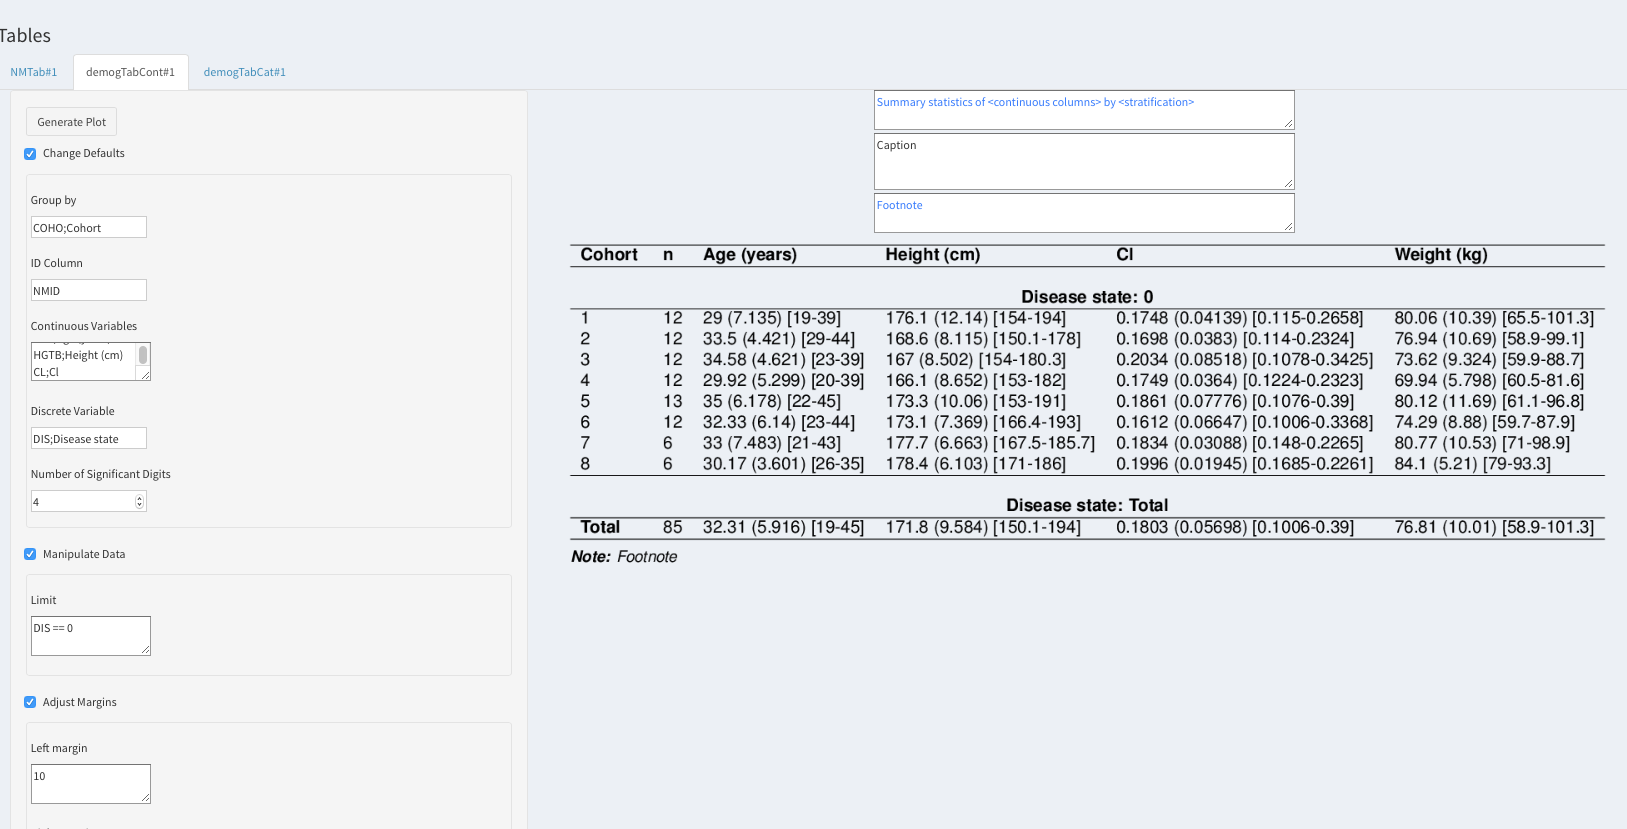
\includegraphics[width=.8\textwidth]{screencaps/26-3-1.png}
\caption{RID: 26 Test ID: 3}
\end{figure}


\begin{figure}[H]
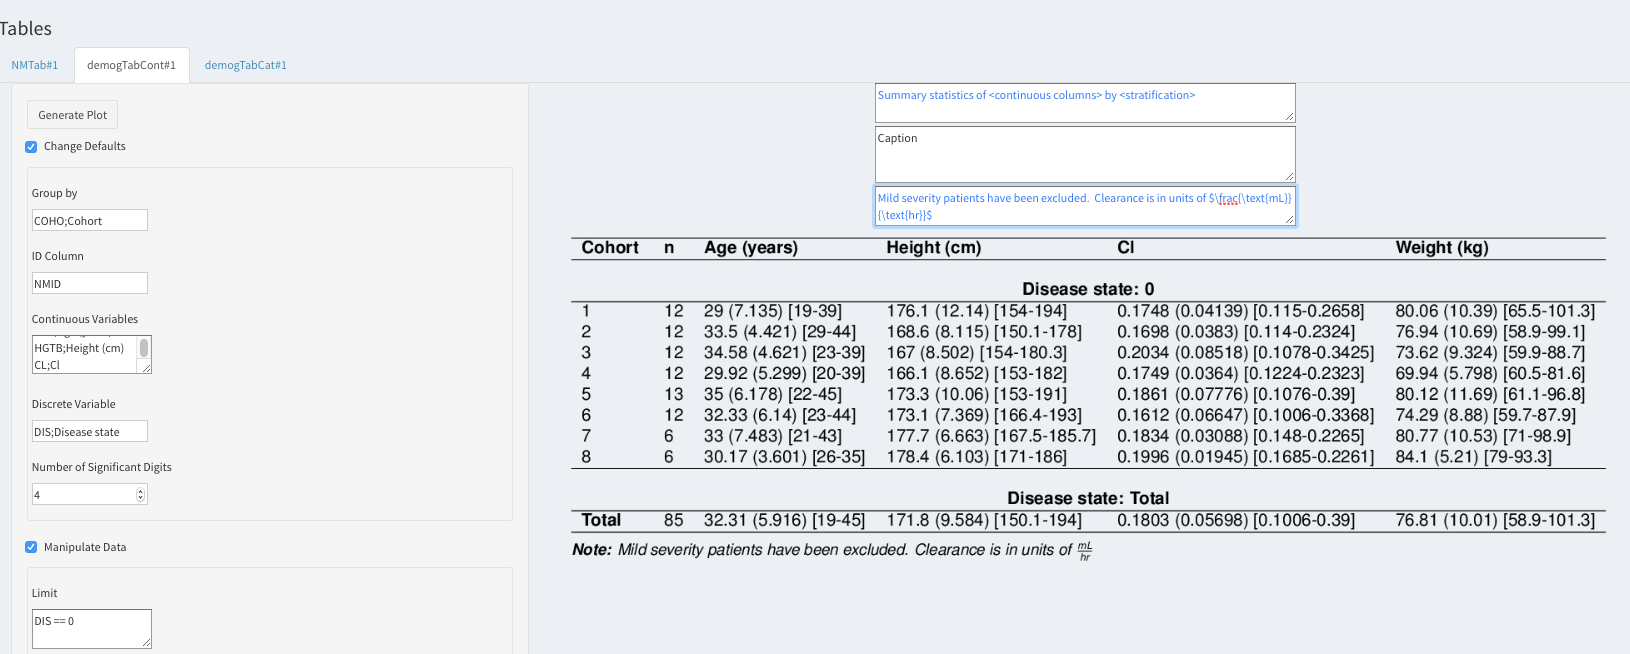
\includegraphics[width=.8\textwidth]{screencaps/26-5-1.png}
\caption{RID: 26 Test ID: 5}
\end{figure}

\begin{figure}[H]
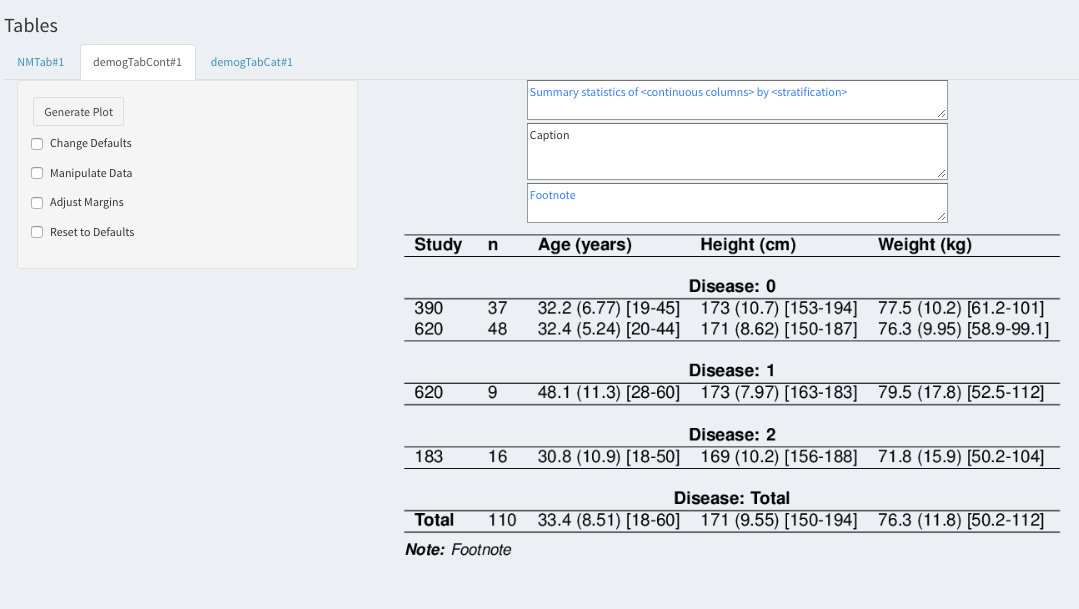
\includegraphics[width=.8\textwidth]{screencaps/26-6-1.png}
\caption{RID: 26 Test ID: 6}
\end{figure}

\begin{figure}[H]
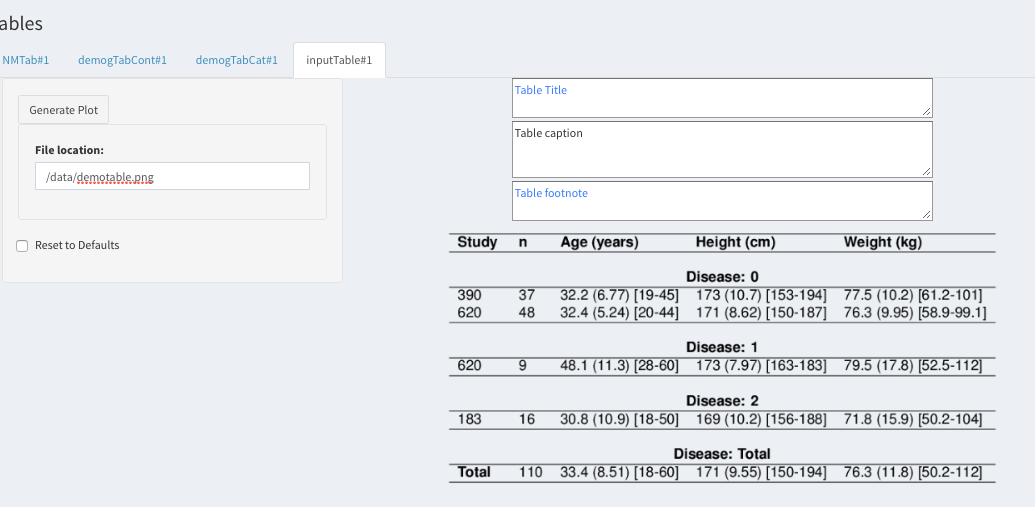
\includegraphics[width=.8\textwidth]{screencaps/27-2-1.png}
\caption{RID: 27 Test ID: 2}
\end{figure}

\begin{figure}[H]
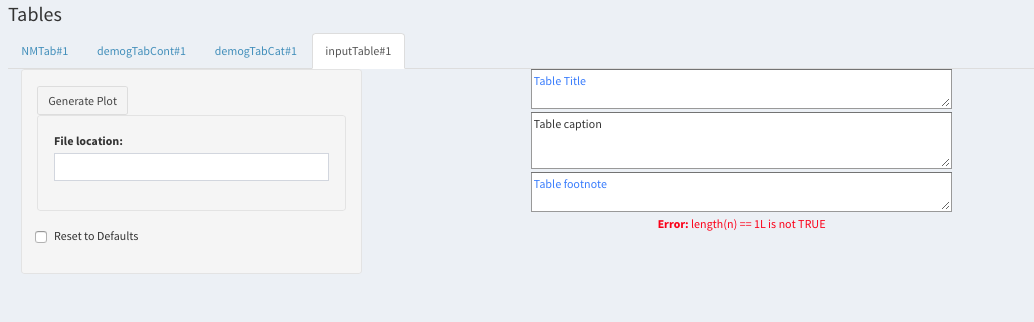
\includegraphics[width=.8\textwidth]{screencaps/27-3-1.png}
\caption{RID: 27 Test ID: 3}
\end{figure}

\begin{figure}[H]
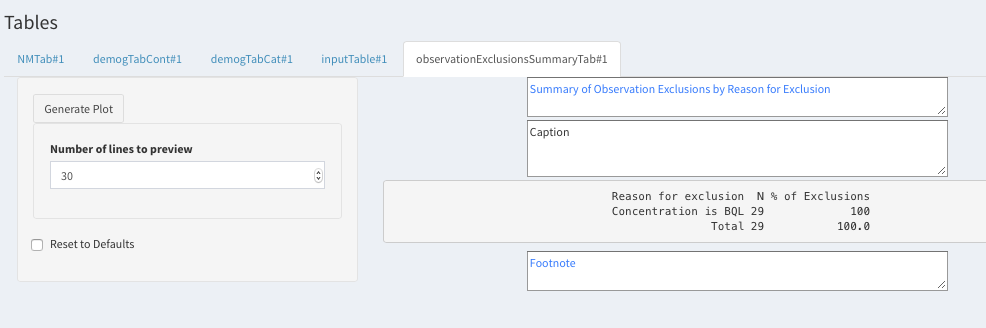
\includegraphics[width=.8\textwidth]{screencaps/28-2-1.png}
\caption{RID: 28 Test ID: 2}
\end{figure}

\begin{figure}[H]
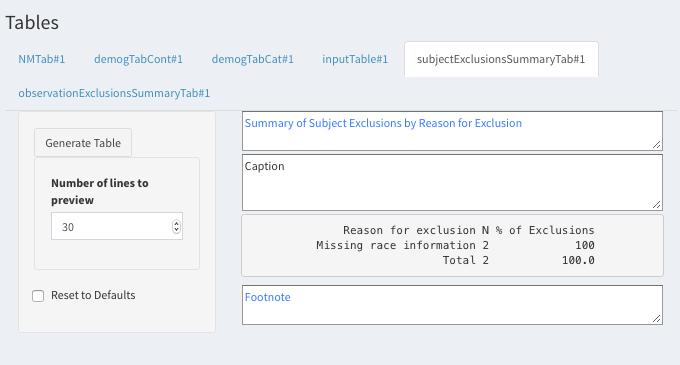
\includegraphics[width=.8\textwidth]{screencaps/29-2-1.png}
\caption{RID: 29 Test ID: 2}
\end{figure}










%% \newpage
%% 
%% \subsection*{Listings}
%% 
%% {\bf RID: 2 Topic ID: 4}
%% 
%% \verbatiminput{listings/asRootpkgSetup.Rout}
%% 
%% \newpage
%% {\bf RID: 2 Topic ID: 5}
%% 
%% \verbatiminput{listings/pkgSetup.Rout}
%%  
\end{document}